\section{Theory and Concepts}

\textbf{Federated Learning Architecture:} The platform follows a coordinator-client model where a central server orchestrates training rounds while hospitals maintain complete data sovereignty. During each round, the coordinator broadcasts the global model to participating clients, who perform local training on private datasets and transmit only encrypted model updates back. The coordinator aggregates these updates using weighted averaging or advanced techniques, producing an improved global model redistributed for the next round. This fundamentally differs from centralized learning by keeping sensitive patient data local, satisfying privacy regulations while enabling collaborative AI development.

\textbf{Aggregation Algorithms:} The platform implements multiple aggregation strategies. FedAvg serves as the baseline using weighted averaging:
\[ w_{global}(t+1) = \sum(n_k / N) \times w_k(t+1) \]
where each hospital's contribution is weighted by dataset size. FedOpt extends this by applying adaptive optimization (Adam, Adagrad) at server level:
\[ w_{global}(t+1) = w_{global}(t) - \eta \times Optimizer(\Delta w_{aggregated}) \]
maintaining momentum terms that smooth inconsistent updates from heterogeneous client datasets. FedMA uses Hungarian algorithm for neuron matching before averaging, achieving higher quality but with 30-50\% overhead. FedProx adds a proximal term enabling partial work from resource-constrained clients.

\textbf{Performance-Aware Weighted Aggregation (PAWA):} Our novel algorithm dynamically computes client weights based on four factors:
\begin{enumerate}
    \item \textbf{Performance Score (40\% weight)} combining validation accuracy and inverse loss:
    \[ \frac{accuracy + \left( \frac{1}{1 + loss} \right)}{2} \]
    \item \textbf{Dataset Size Score (30\% weight)} normalized by total examples:
    \[ \frac{client\_examples}{total\_examples} \]
    \item \textbf{Data Quality Score (20\% weight)} tracking loss improvement consistency over 3 rounds.
    \item \textbf{Progress Score (10\% weight)} measuring recent improvement:
    \[ \frac{previous\_loss - current\_loss}{previous\_loss} \]
\end{enumerate}
Each factor is normalized to [0,1], combined with configurable weights, and clients below performance threshold (default 0.3) are penalized (weight $\times$ 0.1). Final weights use temperature-scaled softmax (default temperature=2.0) for smooth distribution, effectively handling non-IID medical data by prioritizing high-performing, consistent clients.

\textbf{Non-IID Data Challenges:} Medical imaging exhibits severe heterogeneity from demographic variations, equipment differences (scanner manufacturers, protocols), disease prevalence variations, and institutional specializations. These cause weight divergence where local models learn conflicting features. The platform addresses this through PAWA's performance-based weighting, adaptive learning rates in FedOpt, data quality monitoring, and convergence-based dynamic adjustment.

\textbf{Deep Learning Architecture:} The platform uses ResNet-50, a 50-layer residual network employing skip connections that mitigate vanishing gradients in deep networks. Transfer learning leverages ImageNet pretrained weights, adapting general visual features (edges, textures, shapes) to medical domains, significantly reducing training time compared to training from scratch.

\textbf{Core Technologies:} PyTorch provides dynamic computational graphs, automatic differentiation via backpropagation, and GPU acceleration through CUDA. Flower (v1.5) orchestrates federated training with Strategy interface for implementing custom aggregation algorithms, supporting synchronous and asynchronous modes, client sampling, and built-in FedAvg/FedAdam implementations. FastAPI builds the coordinator backend with async/await for concurrent handling, automatic OpenAPI documentation, Pydantic validation, and WebSocket support for real-time monitoring. Next.js 15 powers hospital dashboards with server-side rendering, file-based routing, and React hooks for state management. Docker ensures consistent deployment through containerization, packaging applications with all dependencies into portable images. Supabase provides PostgreSQL database with real-time subscriptions, auto-generated RESTful APIs, row-level security, and JSONB columns for flexible metadata storage.

\textbf{Security Infrastructure:} HTTPS/TLS encrypts communications using RSA 2048-bit key exchange and AES-256-GCM data transmission. Role-based access control (RBAC) restricts functionality through JWT authentication with signed tokens carrying user identity and permissions. WebSocket enables full-duplex communication over persistent connections for real-time monitoring dashboards, reducing latency compared to HTTP polling.

\section{Dataset Description}

\textbf{TB Chest X-ray Dataset:}  
The Tuberculosis Chest X-ray dataset was obtained from Kaggle 
(\href{https://www.kaggle.com/datasets/tawsifurrahman/tuberculosis-tb-chest-xray-dataset}{Kaggle TB Chest X-ray Dataset}). 
It contains 7,000 chest X-ray images categorized as \textit{Normal} or \textit{TB-positive}, sourced from the Shenzhen and Montgomery County datasets. The images are grayscale with resolutions ranging from $512 \times 512$ to $1024 \times 1024$ pixels.

\textbf{Diabetic Retinopathy Dataset:}  
The Diabetic Retinopathy dataset was sourced from Kaggle 
(\href{https://www.kaggle.com/datasets/sovitrath/diabetic-retinopathy-224x224-2019-data}{Kaggle Diabetic Retinopathy Dataset}). 
It consists of 3,662 retinal fundus images collected from screening programs, with five severity levels (0--4) and image resolution of $2048 \times 1536$ pixels.

\textbf{Brain Tumor MRI Dataset:}  
The Brain Tumor MRI dataset was obtained from Kaggle 
(\href{https://www.kaggle.com/datasets/masoudnickparvar/brain-tumor-mri-dataset}{Kaggle Brain Tumor MRI Dataset}). 
It contains 3,624 T1-weighted contrast-enhanced MRI scans classified into Glioma, Meningioma, Pituitary, and No Tumor categories.


\section{Design and Methodology}

\textbf{System Design Principles:}
The proposed federated learning system is designed according to the following core principles:

\begin{enumerate}
    \item \textbf{Privacy-First Architecture:} Raw medical data never leave institutional boundaries; only encrypted model updates are exchanged.
    \item \textbf{Modularity:} Decoupled system components enable independent development, testing, and maintenance.
    \item \textbf{Scalability:} The system supports dynamic onboarding of up to four hospital nodes per training cycle, with extensibility to larger federations.
    \item \textbf{Production Readiness:} Robust error handling, validation checks, and audit logging ensure reliability in real-world deployments.
    \item \textbf{Usability:} Intuitive dashboards and workflows are designed for clinicians and administrators without machine learning expertise.
\end{enumerate}

\textbf{Federated Learning Workflow:}
Model training proceeds iteratively across multiple federated rounds, following five structured phases:

\begin{enumerate}
    \item \textit{Initialization:} The coordinator initializes a ResNet-50 model with ImageNet-pretrained weights, stores the model in Supabase, and securely distributes the initial parameters to registered hospital clients.
    
    \item \textit{Local Training:} Each hospital performs local training using its private medical imaging dataset for 5--10 epochs. Model weight updates are computed as the difference between updated and received parameters and are encrypted prior to transmission.
    
    \item \textit{Aggregation:} The coordinator validates received updates (dimension consistency, NaN detection) and applies the selected aggregation algorithm (FedAvg, FedOpt, FedMA, FedProx, or PAWA). In the PAWA strategy, client weights are dynamically computed using validation performance, dataset size, data quality indicators, and training progress. A temperature-scaled softmax function is applied to obtain stable aggregation weights before performing weighted averaging.
    
    \item \textit{Distribution:} The updated global model is broadcast to all participating hospitals. Training metrics and convergence statistics are streamed to monitoring dashboards via WebSocket connections.
    
    \item \textit{Convergence Check:} Training continues until the target performance threshold (95\% of centralized baseline accuracy) is reached or a predefined maximum number of rounds is completed, after which the final model is exported.
\end{enumerate}

\textbf{Preprocessing Pipeline:}
A standardized preprocessing pipeline is enforced across all hospitals to ensure consistency:

\begin{enumerate}
    \item Image loading using Pillow with support for JPEG, PNG, and DICOM formats.
    \item Resizing to $224 \times 224$ using bicubic interpolation.
    \item Intensity normalization to $[0,1]$ followed by ImageNet normalization ($\mu=[0.485, 0.456, 0.406]$, $\sigma=[0.229, 0.224, 0.225]$).
    \item Removal of EXIF metadata and textual overlays to prevent privacy leakage.
    \item Data augmentation including $\pm15^\circ$ rotations, horizontal flips, brightness and contrast variations ($\pm20\%$), and random cropping.
    \item Automated quality checks for corrupted files, resolution constraints, and statistical distribution validation.
\end{enumerate}

\textbf{Communication Protocol:}
Two complementary communication channels are implemented:

\begin{enumerate}
    \item \textbf{REST API (FastAPI):} Secure endpoints include \texttt{/api/submit\_update} for uploading encrypted model updates and \texttt{/api/get\_model} for retrieving the latest global model. Authentication is enforced using JWT tokens, and payloads are transmitted as JSON objects with Base64-encoded tensors.
    
    \item \textbf{WebSocket Channel:} A persistent WebSocket connection enables real-time dissemination of training progress, round-level metrics, client status updates, and heartbeat monitoring.
\end{enumerate}

\textbf{Security Implementation:}
The system incorporates multi-layered security mechanisms, including TLS~1.3 encryption with certificate pinning, JWT-based authentication with 24-hour expiration and refresh rotation, bcrypt password hashing, role-based access control (RBAC), and immutable audit logging of all model transmissions with automated anomaly alerts.

\textbf{Monitoring and Observability:}
Comprehensive monitoring capabilities include global and per-client accuracy and loss trends, training time, communication overhead, convergence rates, system health indicators (GPU utilization, latency, connectivity), and real-time dashboards updated via WebSockets. For PAWA, additional visualizations display client weight evolution, factor-wise contribution analysis, and threshold violation alerts.

\section{System Architecture}

\textbf{Three-Tier Architecture:} 
The proposed system follows a three-tier architectural design that distinctly separates hospital-side model training, centralized coordination and aggregation, and persistent data management. This separation enhances scalability, security, modularity, and ease of system maintenance.


\textit{Tier 1 -- Hospital Clients:} Dockerized training environments execute PyTorch-based local learning. Each hospital hosts a Next.js web application for interaction, local dataset management, and real-time communication with the coordinator.

\textit{Tier 2 -- Coordinator Server:} A FastAPI-based coordinator deployed on the Vercel cloud orchestrates federated rounds using the Flower framework. The server integrates a multi-algorithm aggregation engine supporting FedAvg, FedOpt, FedMA, FedProx, and PAWA, and maintains persistent WebSocket connections for monitoring and control.

\textit{Tier 3 -- Data Layer:} Supabase PostgreSQL manages model versioning, metadata storage, audit logs, authentication, and role management. Real-time subscriptions enable live updates to monitoring dashboards.

\textbf{Component Interactions:}
\begin{enumerate}
    \item Secure client registration via authenticated WebSocket connections.
    \item Distribution of initial model parameters and training configurations.
    \item Local model training within hospital environments.
    \item Encrypted submission of model updates and validation metrics.
    \item Aggregation using PAWA or baseline algorithms and persistent model storage.
    \item Real-time distribution of updated models and aggregation insights.
    \item Continuous monitoring and visualization of training progress.
\end{enumerate}

\textbf{Scalability Design:}
Serverless deployment on Vercel enables automatic scaling based on workload. WebSocket connections are load-balanced across instances, while Supabase supports high concurrency and real-time data streaming. Docker-based clients ensure consistent deployment, and asynchronous aggregation allows partial client participation. PostgreSQL partitioning and archival strategies are employed to manage large audit logs and historical model versions.

\begin{figure}[H]
    \centering
    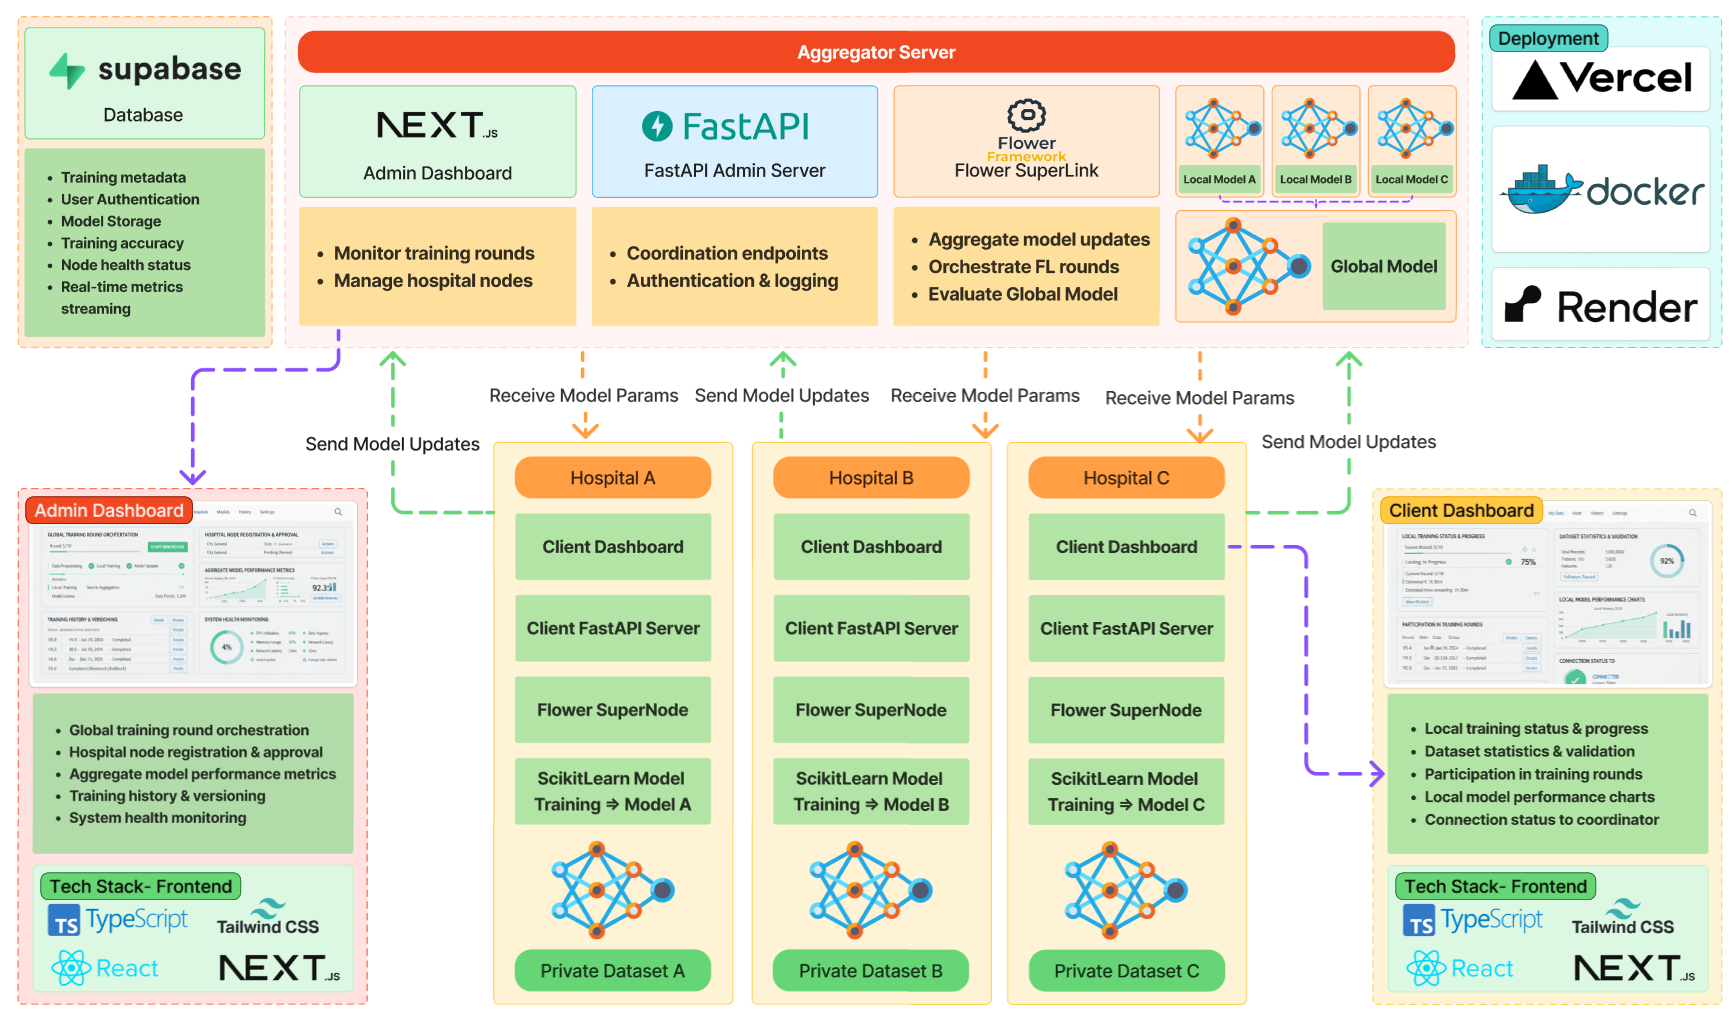
\includegraphics[width=0.9\textwidth]{images/fedml-architecture.png}
    \caption{Federated Learning System Architecture}
    \label{fig:fedml_architecture}
\end{figure}

\section{Tools and APIs}

\textbf{Core Frameworks:} Flower v1.5 for federated orchestration with custom PAWA Strategy class, PyTorch v2.0 for deep learning with GPU support, FastAPI v0.104 for async web framework, Next.js 15 for React-based frontend, Docker v24.0 for containerization.

\textbf{Data Processing:} NumPy v1.24+ for numerical operations, Pillow v10.0+ for image processing, torchvision v0.15+ for pretrained ResNet-50 and augmentation, pandas for metrics logging.

\textbf{Database and Storage:} Supabase providing PostgreSQL v14+ with real-time subscriptions and RESTful APIs, storing model versions, audit logs, PAWA weight histories, and performance metrics.

\textbf{Deployment:} Vercel for serverless FastAPI coordinator and Next.js dashboards, Render for alternative backend hosting, Docker Hub for client application distribution.

\textbf{Key APIs:} Flower API with \texttt{start\_server()}, \texttt{start\_client()}, custom \texttt{PAWAStrategy} class overriding \texttt{aggregate\_fit()} with performance-aware weight computation; FastAPI endpoints for model submission and retrieval; Supabase REST API for automatic database CRUD; External resources including Kaggle datasets and ImageNet weights from PyTorch model zoo.

\textbf{Security Tools:} pyjwt for token generation, jsonwebtoken for validation, bcrypt for password hashing, TLS 1.3 for transport encryption.

\section{Summary}

The proposed system integrates federated learning with modern web technologies to enable production-ready healthcare AI. It employs FedAvg (baseline), FedOpt (adaptive), and the novel PAWA algorithm, which dynamically weights clients based on performance (40\%), dataset size (30\%), data quality (20\%), and progress (10\%) using temperature-scaled softmax. ResNet-50 models with ImageNet transfer learning classify medical images across TB Chest X-rays (7,000), Diabetic Retinopathy (3,662), and Brain Tumor MRI (3,624), distributed across 4 hospitals with non-IID data.

A three-tier architecture separates hospital clients (Docker + PyTorch), coordinator server (Flower + FastAPI with PAWA), and data layer (Supabase for models and audit logs). Communication uses HTTPS REST and WebSocket, secured with TLS and JWT. Hospitals train locally for 5-10 epochs, submit encrypted updates, and the coordinator aggregates using PAWA’s multi-factor weighting.

Standardized preprocessing (224$\times$224 resizing, ImageNet normalization, metadata stripping, augmentation) ensures consistency. The technology stack—Flower, PyTorch, FastAPI, Next.js, Docker, Supabase—supports scalability, security, and monitoring. PAWA effectively handles non-IID medical data, prioritizing consistent high-performing clients while maintaining fairness, addressing key challenges in collaborative healthcare AI.
